\documentclass[12pt]{article}
\usepackage{amsmath}
\usepackage{graphicx}
\usepackage{hyperref}
\usepackage[utf8]{inputenc}
\usepackage{geometry}
\usepackage{mathtools}
\usepackage{empheq}
\usepackage{listings}
\usepackage{xcolor}
\usepackage{minted}
\usepackage{svg}


\definecolor{LightGray}{gray}{0.9}

\graphicspath{ {./assets/} }
\geometry{margin=0.6in}

\title{CHEN 461 HW 6}
\author{Mark Levchenko}
\date{January 2023}

\begin{document}


\begin{enumerate}

% Problem 1 %%%%%%%%%%%%%%%%%%%%%%%%%%%%%%%%%%%%%%%%%%%%%%%%%%%%%%%%%%%%%%%%%%%%%%%%%%%
\newpage
\item Problem 7.7
\begin{enumerate}
    \item 
    \begin{align*}
        \frac{dC_R}{dt} &= -\frac{F}{V} C_R - k_1 C_R - k_3 C_R^2 + \frac{F}{V} C_{R,in} \\
        \frac{dC_P}{dt} &= -\frac{F}{V} C_P - k_2 C_P + k_1 C_R \\
        \intertext{At steady state}
        0 &= -\frac{F_s}{V} C_R - k_1 C_R - k_3 C_R^2 + \frac{F_s}{V} C_{R,in,s} \\
        0 &= -\frac{F_s}{V} C_P - k_2 C_P + k_1 C_R \\
        & F_s = 21 \\
        & C_{R,in,s} = 5.5 \\
        & V = 1 \\
        & k_1 = 50 \\
        & k_2 = 54 \\
        & k_3 = 4 \\
        \intertext{Solve the system of equations}
        \Aboxed{C_{R,s} &= 1.5} \\
        \Aboxed{C_{P,s} &= 1}
    \end{align*}
    \item 
    \begin{align*}
        \intertext{Linearize in deviation form}
        \frac{dC_R}{dt} &= f_1(x, u) \\
        \frac{dC_P}{dt} &= f_2(x, u) \\
        A &= \begin{bmatrix}
            \frac{\partial f_1}{\partial C_R}(x_s, u_s) & \frac{\partial f_1}{\partial C_P}(x_s, u_s) \\
            \frac{\partial f_2}{\partial C_R}(x_s, u_s) & \frac{\partial f_2}{\partial C_P}(x_s, u_s) \\
        \end{bmatrix} \\
        A &= \begin{bmatrix}
            -\left(\frac{F_s}{V} + k_1 + 2 k_3 C_{R,s}\right) & 0 \\
            k_1 & -\left(\frac{F_s}{V} + k_2\right) \\
        \end{bmatrix} \\
        B &= \begin{bmatrix}
            \frac{\partial f_1}{\partial C_{R,in}}(x_s, u_s) & \frac{\partial f_1}{\partial F}(x_s, u_s) \\
            \frac{\partial f_2}{\partial C_{R,in}}(x_s, u_s) & \frac{\partial f_2}{\partial F}(x_s, u_s) \\
        \end{bmatrix} \\
        B &= \begin{bmatrix}
            F_s & C_{R,in,s} - C_{R,s} \\
            0 & -C_{P,s} \\
        \end{bmatrix} \\
        A &= \begin{bmatrix}
            -\left(\frac{21}{1} + 50 + 2 \cdot 4  \cdot 1.5 \right) & 0 \\
            50 & -\left(\frac{21}{1} + 54\right) \\
        \end{bmatrix} \\
        A &= \begin{bmatrix}
            -83 & 0 \\
            50 & -75 \\
        \end{bmatrix} \\
        B &= \begin{bmatrix}
            21 & 5.5 - 1.5 \\
            0 & -1 \\
        \end{bmatrix} \\
        B &= \begin{bmatrix}
            21 & 4 \\
            0 & -1 \\
        \end{bmatrix} \\
        c &= \begin{bmatrix}
            0 & 1 \\
        \end{bmatrix} \\
        d &= 0 \\
        \intertext{Linearized system}
        \frac{d}{dt} \begin{bmatrix}
            \overline{C}_R \\
            \overline{C}_P \\
        \end{bmatrix} &= \begin{bmatrix}
            -83 & 0 \\
            50 & -75 \\
        \end{bmatrix} \begin{bmatrix}
            \overline{C}_R \\
            \overline{C}_P \\
        \end{bmatrix} + \begin{bmatrix}
            21 & 4 \\
            0 & -1 \\
        \end{bmatrix} \begin{bmatrix}
            \overline{C}_{R,in} \\
            \overline{F} \\
        \end{bmatrix} \\
        y &= \overline{C}_P \\
        \intertext{Check asymptotic stability}
        0 &= \begin{bmatrix}
            \lambda-(-83) & 0 \\
            50 & \lambda-(-75) \\
        \end{bmatrix} \\
        \lambda &= -75, -83 \\
        \intertext{Eigenvalues are negative, and so the system is asymptotically stable.}
    \end{align*}
    \item 
    \begin{align*}
        \intertext{Non-linear system}
        \frac{dC_R}{dt} &= -\frac{F}{V} C_R - k_1 C_R - k_3 C_R^2 + \frac{F}{V} C_{R,in} \\
        \frac{dC_P}{dt} &= -\frac{F}{V} C_P - k_2 C_P + k_1 C_R \\
        \intertext{Solve the system of ODEs with the following parameters}
        & F = 28 \\
        & C_{R,in} = 5.5 \\
        & V = 1 \\
        & k_1 = 50 \\
        & k_2 = 54 \\
        & k_3 = 4 \\
        \intertext{Linear system}
        \frac{d\overline{C}_R}{dt} &= -83 \overline{C}_R + 21 \overline{C}_{R,in} + 4 \overline{F} \\
        \frac{d\overline{C}_P}{dt} &= 50 \overline{C}_R - 75 \overline{C}_P - \overline{F} \\
        \intertext{Solve the system of ODEs with the following parameters}
        & \overline{F} = 7 \\
        & \overline{C}_{R,in} = 0 \\
        & k_1 = 50 \\
        & k_2 = 54 \\
        & k_3 = 4 \\
    \end{align*}

    $C_R$ Plot:

    \begin{center}
        \includesvg[width=0.8\textwidth]{assets/p1_r.svg}
    \end{center}

    $C_P$ Plot:

    \begin{center}
        \includesvg[width=0.8\textwidth]{assets/p1_p.svg}
    \end{center}
\end{enumerate}


% Problem 2 %%%%%%%%%%%%%%%%%%%%%%%%%%%%%%%%%%%%%%%%%%%%%%%%%%%%%%%%%%%%%%%%%%%%%%%%%%%
\newpage
\item Problem 6.9
    \begin{enumerate}
        \item 
        \begin{align*}
            \frac{dx_1}{dt} &= -83x_1 + 21u_1 + 4u_2 \\  
            \frac{dx_2}{dt} &= 50x_1 - 75x_2 - u_2 \\
            sX_1 &= -83X_1 + 21U_1 + 4U_2 \\
            X_1 &= \frac{21}{s+83} U_1 + \frac{4}{s+83} U_2 \\
            sX_2 &= 50X_1 - 75X_2 - U_2 \\
            X_2 (s+75) &= 50X_1 - U_2 \\
            X_2 (s+75) &= 50\left(\frac{21}{s+83} U_1 + \frac{4}{s+83} U_2\right) - U_2 \\
            X_2 (s+75) &= \frac{1050}{s+83} U_1 + \frac{117-s}{s+83} U_2 \\
            X_2 &= \frac{1050}{\left(s+83\right)\left(s+75\right)} U_1 + \frac{117-s}{\left(s+83\right)\left(s+75\right)} U_2 \\
            \Aboxed{G_1(s) &= \frac{1050}{\left(s+83\right)\left(s+75\right)}} \\
            \Aboxed{G_2(s) &= \frac{117-s}{\left(s+83\right)\left(s+75\right)}}
        \end{align*}

        \begin{center}
            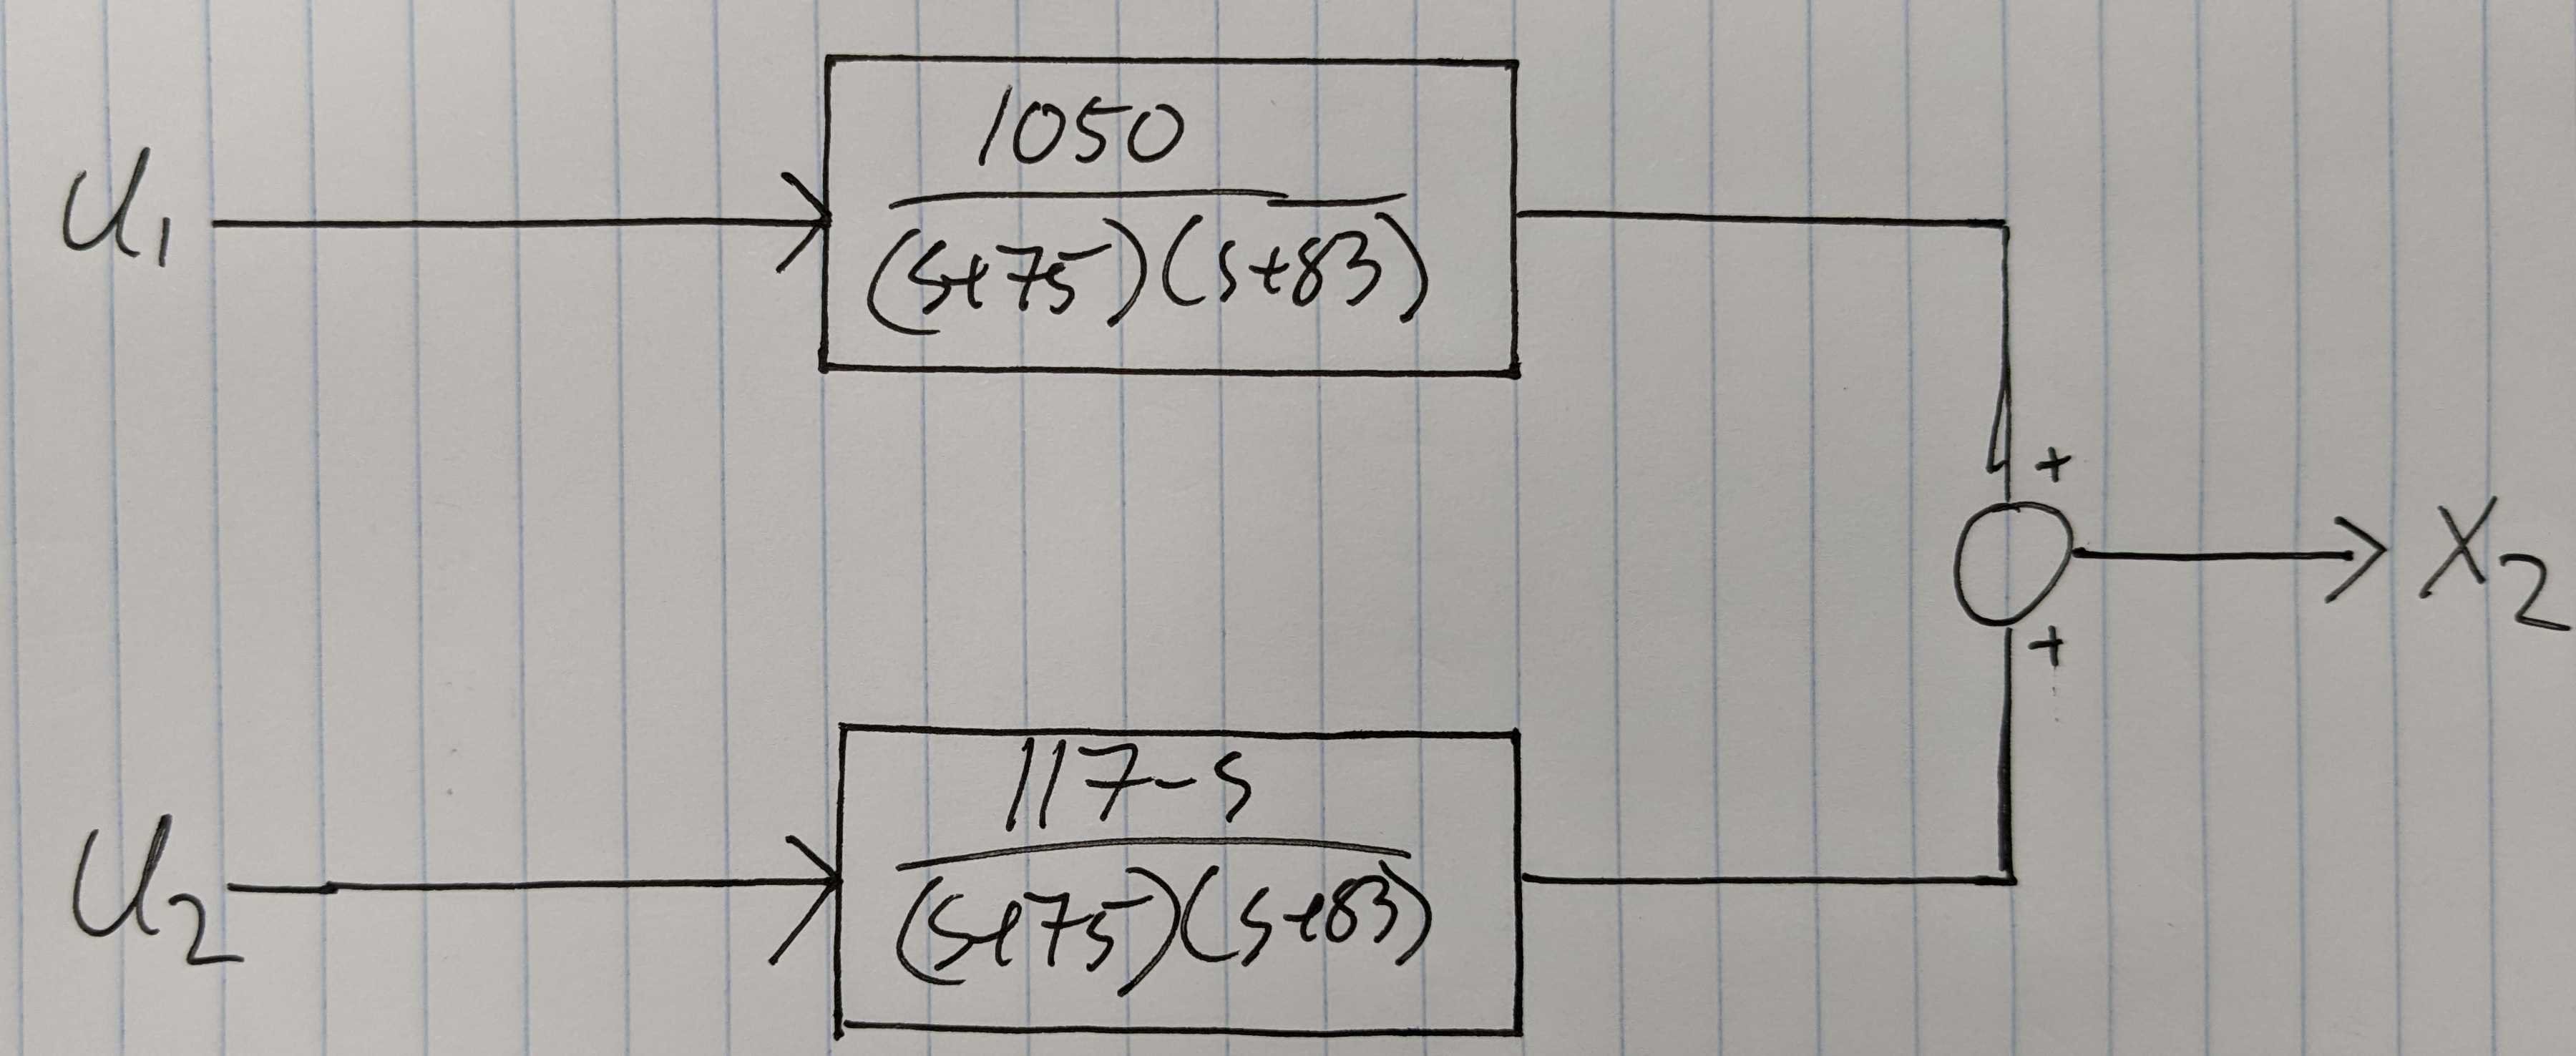
\includegraphics[width=0.8\textwidth]{assets/block_diagram.jpg}
        \end{center}
        \item 
        
        $x_1$ Plot:

        \includesvg{assets/p2_x1.svg}

        $x_2$ Plot:
        
        \includesvg{assets/p2_x2.svg}
    \end{enumerate}


\end{enumerate}
\end{document}